\section{Simulation Analysis Agent System}

\begin{figure*}[H]

      \centering
    
      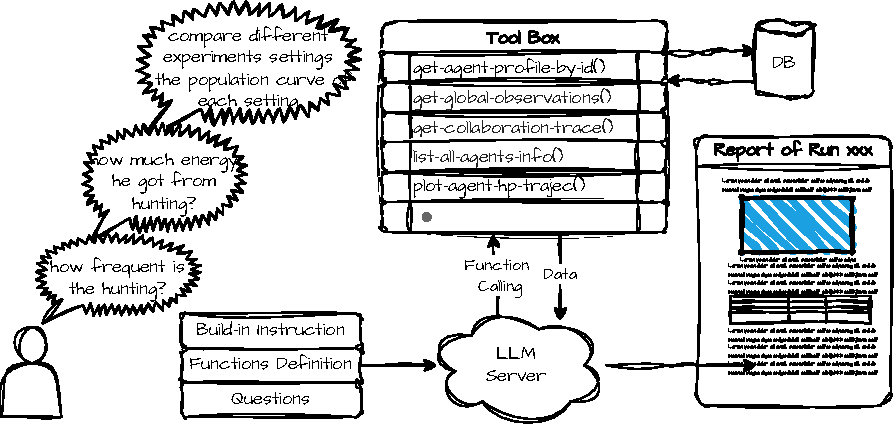
\includegraphics[width=0.9\textwidth]{figures/Post-Processing-Analysis-System.drawio.pdf}
    
      \caption{Overview of the post-processing analysis system architecture, showing the integration of RAG techniques, agent behavior logging, and structured reporting components. The diagram illustrates how raw simulation data is transformed into actionable insights through various analysis pipelines and iterative querying.}
      
      \label{fig:post-processing}
    
\end{figure*}

The Simulation Analysis Agent System is a comprehensive post-processing analysis framework for the Morality-AI simulation environment. It is engineered to distill actionable insights and facilitate in-depth investigation of simulation outcomes using a Retrieval-Augmented Generation (RAG) approach.

This system is based on the existing code agent tools like Github Copilot\footnote{\url{https://github.com/features/copilot}} and Cursor\footnote{\url{https://www.cursor.com/}}, etc, to manage the file calling system. During usage, one simply provides our analysis agent instruction file, the tool calling code file, and gives an experiment run identifier. The system will then automatically extract the experiment data and generate the analysis report, and provide interactive Q\&A.

This system consists of three primary components:
\begin{itemize}
    \item A \textbf{Simulation Analysis Agent} that orchestrates the analysis.
    \item An \textbf{Analytical Tool Suite} providing data processing and visualization functions.
    \item A \textbf{Reporting System} that generates structured outputs.
\end{itemize}

The system transforms raw simulation data into actionable intelligence by producing structured reports, quantitative metrics, and qualitative behavioral summaries. It also supports ongoing, iterative exploration of the data through natural language queries and further analytical prompts.

\subsection{Components}

The system is architected around three tightly integrated components:

\subsubsection{Simulation Analysis Agent}

The \textbf{Simulation Analysis Agent} is the central component that orchestrates the entire analytical workflow.

\begin{itemize}
    \item \textbf{Core Functions:}
    \begin{itemize}
        \item \textbf{Tool Calling Orchestration:} Coordinates the retrieval and transformation of simulation data by leveraging the Analytical Tool Suite. It accesses specific data slices such as agent profiles, global event logs, and collaboration traces.
        \item \textbf{RAG Interpretation:} Employs customized functions for efficient Retrieval-Augmented Generation to interpret and analyze simulation data.
        \item \textbf{Analysis Report Generation:} Synthesizes hierarchical analytical artifacts, including global summaries and lineage-specific analyses, combining quantitative metrics with qualitative behavioral insights.
        \item \textbf{Interactive Exploration:} Supports iterative, natural language-driven queries, enabling researchers to probe deeper into specific events, patterns, or hypotheses beyond initial report generation.
    \end{itemize}
    \item \textbf{How it Works:}
    Upon receiving a simulation run identifier, the agent initiates a multi-stage pipeline. It intelligently calls upon the various tools in the Analytical Tool Suite to fetch, process, and analyze data, then synthesizes this information to generate reports or respond to specific user queries.
\end{itemize}

\subsubsection{Analytical Tool Suite}

The \textbf{Analytical Tool Suite} (referred to as Analytical Framework in the original documentation) underpins the system's analytical capabilities through a robust, tool-driven interface.

\begin{itemize}
    \item \textbf{Core Functions:}
    \begin{itemize}
        \item Provides a library of modular, callable functions that abstract complex data queries and analytical routines.
        \item \textbf{Information Extraction:} Offers tools for retrieving diverse data sets. Examples include:
        \begin{itemize}
            \item \texttt{GetAgentProfile}: Retrieves comprehensive data for specified agents (state, family, actions, outcomes).
            \item \texttt{GetPopulationData}: Compiles and aggregates population-wide statistics (demographics, archetype distributions).
            \item \texttt{GetGlobalObservations}: Fetches or queries simulation-wide event logs (e.g., fights, robberies).
            \item \texttt{GetCollaborationTrace}: Extracts and summarizes data on cooperative interactions.
        \end{itemize}
        \item \textbf{Data Processing and Aggregation:} Includes functions for transforming and summarizing raw data, supporting both population-level and individual-level analyses.
        \item \textbf{Visualization:} Enables automated generation of plots, graphs, and statistical summaries to elucidate dynamic patterns and relationships. Examples include:
        \begin{itemize}
            \item \texttt{PlotAgentHPTrajectory}: Generates time-series plots of Health Point (HP) trajectories.
            \item \texttt{PlotPopulationComposition}: Visualizes the distribution and temporal changes of agent archetypes.
            \item \texttt{PlotMortalityAnalytics}: Produces visualizations of mortality patterns.
        \end{itemize}
        \item \textbf{Table Generation:} Offers functions like \texttt{FormatDataIntoTable} to structure extracted data into formatted tables for reports.
    \end{itemize}
    \item \textbf{How it Works:}
    This suite provides a collection of callable tools that the Simulation Analysis Agent utilizes to access, process, and visualize simulation data. These tools enable both macroscopic (population-level) and microscopic (individual-level) exploration of the simulation outcomes.
\end{itemize}

\subsubsection{Reporting System}

The \textbf{Reporting System} translates analytical results into structured, reproducible outputs.

\begin{itemize}
    \item \textbf{Core Functions:}
    \begin{itemize}
        \item \textbf{Structured Output Generation:} Produces standardized reports and visualizations for each simulation run.
        \item \textbf{Main Simulation Report:} Generates a comprehensive overview including an initial summary, population statistics, social dynamics analysis, key metrics, visualizations, and an index of detailed agent reports.
        \item \textbf{Agent-Specific Reports:} Creates detailed profiles for key agents (e.g., ancestors and significant descendants), covering state attributes, behavioral summaries, social interaction patterns, reproductive metrics, and qualitative analyses.
        \item \textbf{Visualization Suite:} Automatically produces a variety of visualizations, such as time-series plots (population composition, HP trajectories), network graphs (social connections, resource sharing), and statistical distributions (age-at-death, resource accumulation).
    \end{itemize}
    \item \textbf{How it Works:}
    For each analyzed simulation run, the Reporting System generates a standardized directory structure. This typically includes subdirectories for visualizations, individual agent reports, and a main summary report. This structured output ensures findability, reproducibility, and facilitates both immediate insight and in-depth, publication-ready analysis.
\end{itemize}

\subsection{Analysis Capabilities}

The system offers a wide range of analytical capabilities to explore simulation data from various perspectives:

\begin{itemize}
    \item \textbf{Population-Level Analysis}
    \begin{itemize}
        \item \textbf{Demographic Tracking:} Monitoring population size, age distribution, and mortality rates.
        \item \textbf{Archetype Distribution:} Analyzing the prevalence and evolution of behavioral archetypes within the population.
        \item \textbf{Mortality Patterns:} Tracking causes of death, age-at-death distributions, and survival rates.
    \end{itemize}

    \item \textbf{Individual Agent Analysis}
    \begin{itemize}
        \item \textbf{Agent Profiling:} Comprehensively tracking individual agent states, attributes, and actions over time.
        \item \textbf{Behavioral Tracking:} Analyzing decision-making patterns and the evolution of individual strategies.
        \item \textbf{Performance Metrics:} Evaluating individual agent success through various defined metrics.
    \end{itemize}

    \item \textbf{Social Dynamics Analysis}
    \begin{itemize}
        \item \textbf{Interaction Patterns:} Analyzing the frequency and nature of cooperation, conflict, and communication events between agents.
        \item \textbf{Network Analysis:} Mapping social connection networks, resource-sharing networks, and communication flows.
        \item \textbf{Communication Flows:} Tracking information exchange among agents and its impact on collective behavior.
        \item \textbf{Resource Sharing:} Analyzing patterns of resource allocation and distribution within the population.
        \item \textbf{Conflict Analysis:} Examining conflict events such as fight initiations and robbery attempts, along with their outcomes.
    \end{itemize}

    \item \textbf{Evolutionary Analysis}
    \begin{itemize}
        \item \textbf{Lineage Tracking:} Following agent lineages from initial ancestors through successive generations of descendants.
        \item \textbf{Ancestor Identification:} Detecting founder agents and assessing their long-term impact on the population.
        \item \textbf{Success Metrics:} Evaluating reproductive success and the survival rates of different lineages.
        \item \textbf{Behavioral Inheritance:} Analyzing the persistence and modification of traits and behaviors across generations.
    \end{itemize}
\end{itemize}

% \begin{figure}[H]
%     \centering
%     \begin{subfigure}[b]{0.48\columnwidth}
%         \centering
%         
\includegraphics[width=\textwidth,height=0.3\textheight,keepaspectratio]{appendix_figures/sim_analysis_agent/main_report1.png}
%         \caption{Main Report Example Screenshot (Part 1)}
%         \label{fig:main_report1}
%     \end{subfigure}
%     \hfill
%     \begin{subfigure}[b]{0.48\columnwidth}
%         \centering
%         
\includegraphics[width=\textwidth,height=0.3\textheight,keepaspectratio]{appendix_figures/sim_analysis_agent/main_report2.png}
%         \caption{Main Report Example Screenshot (Part 2)}
%         \label{fig:main_report2}
%     \end{subfigure}
%     \caption{Main Analysis Report Visualizations}
%     \label{fig:main_reports}
% \end{figure}



% \begin{figure}[H]
%     \centering
%     \begin{subfigure}[b]{0.48\columnwidth}
%         \centering
%         
\includegraphics[width=\textwidth,height=0.35\textheight,keepaspectratio]{appendix_figures/sim_analysis_agent/agent5_report1.png}
%         \caption{Agent Specific Report Example Screenshot (Part 1)}
%         \label{fig:agent5_report1}
%     \end{subfigure}
%     \hfill
%     \begin{subfigure}[b]{0.48\columnwidth}
%         \centering
%         
\includegraphics[width=\textwidth,height=0.35\textheight,keepaspectratio]{appendix_figures/sim_analysis_agent/agent5_report2.png}
%         \caption{Agent Specific Report Example Screenshot (Part 2)}
%         \label{fig:agent5_report2}
%     \end{subfigure}
%     \caption{Agent-Specific Analysis Report Visualizations}
%     \label{fig:agent_reports}
% \end{figure}

